% Bài luận triết học: Chủ nghĩa duy vật cổ đại
% Biên dịch: XeLaTeX hoặc LuaLaTeX (hỗ trợ tiếng Việt Unicode)

\documentclass[14pt,a4paper]{extarticle}

% Gói tiếng Việt (Unicode)
\usepackage{fontspec}
\usepackage{polyglossia}
\setmainlanguage{vietnamese}
\setmainfont{Times New Roman}

% Layout và hình thức
\usepackage[margin=2.5cm]{geometry}
\usepackage{graphicx}
\usepackage{framed}
\usepackage[normalem]{ulem}
\usepackage{indentfirst}
\usepackage{setspace}
\onehalfspacing
\setlength{\parindent}{1.25cm}
\usepackage{tocloft}
\setlength{\cftsecnumwidth}{5.2em}
\setlength{\cftsubsecnumwidth}{2.8em}
\setlength{\cftsubsubsecnumwidth}{4em}
\renewcommand{\thesection}{Chương \arabic{section}\quad}
\renewcommand{\thesubsection}{\arabic{section}.\arabic{subsection}}
\renewcommand{\thesubsubsection}{\arabic{section}.\arabic{subsection}.\arabic{subsubsection}}

% Trích dẫn và tài liệu tham khảo
\usepackage{csquotes}
\DeclareQuoteStyle{vietnamese}
  {\guillemotleft}{\guillemotright}
  {\textquotedblleft}{\textquotedblright}
\usepackage[backend=biber,style=ieee,sorting=none,bibencoding=utf8,giveninits=false]{biblatex}
\addbibresource{references.bib}
\DeclareFieldFormat{labelnumberwidth}{\mkbibbrackets{#1}\addperiod}
\ExecuteBibliographyOptions{giveninits=false}
\setlength{\emergencystretch}{5em}
\AtBeginBibliography{\sloppy}

\DeclareBibliographyDriver{book}{%
  \usebibmacro{bibindex}%
  \usebibmacro{begentry}%
  \printnames{author}%
  \setunit{\addcomma\space}%
  \printfield{year}%
  \setunit{\addcomma\space}%
  \printfield{title}%
  \setunit{\addcomma\space}%
  \printlist{publisher}%
  \iflistundef{location}{}{\setunit{\addcomma\space}\printlist{location}}%
  \usebibmacro{finentry}%
}

\DeclareBibliographyDriver{incollection}{%
  \usebibmacro{bibindex}%
  \usebibmacro{begentry}%
  \printnames{author}%
  \setunit{\addcomma\space}%
  \printfield{year}%
  \setunit{\addcomma\space}%
  \printfield{title}%
  \setunit{\addcomma\space}%
  \printfield{booktitle}%
  \setunit{\addcomma\space}%
  \printlist{publisher}%
  \usebibmacro{finentry}%
}

\DeclareBibliographyDriver{periodical}{%
  \usebibmacro{bibindex}%
  \usebibmacro{begentry}%
  \printfield{title}%
  \setunit{\addcomma\space}%
  \printlist{publisher}%
  \iflistundef{location}{}{\setunit{\addcomma\space}\printlist{location}}%
  \usebibmacro{finentry}%
}

\usepackage[unicode,colorlinks=true,linkcolor=blue,urlcolor=blue,citecolor=blue,
  bookmarks=true,bookmarksopen=true,bookmarksnumbered=true,bookmarksdepth=3,
  pdfencoding=unicode]{hyperref}
\usepackage[open,numbered,depth=3]{bookmark}

% Thông tin bìa (có thể sửa trực tiếp tại đây)
\newcommand{\hocphan}{Triết học}
\newcommand{\tenduan}{Chủ nghĩa duy vật cổ đại: giá trị triết học và giới hạn lịch sử}
\newcommand{\giangvien}{Phạm Quốc Hương}
\newcommand{\hocvien}{Nông Văn Tình}
\newcommand{\mahocvien}{8480101250028}
\newcommand{\lop}{Khoa học máy tính}
\newcommand{\malop}{25MCS2}
\newcommand{\nganh}{Khoa học máy tính}
\newcommand{\manganh}{8480101}
\newcommand{\thangnam}{.... / .....}
\newcommand{\noidungnghiencuu}{\tenduan}

\begin{document}

%==============================================================================
% BÌA 1 (trang 1 - theo mẫu BIA DO AN CUOI MON MCS.docx)
%==============================================================================
\thispagestyle{empty}
\begin{center}
\vspace*{0.3cm}
{\fontsize{14}{18}\selectfont\bfseries BỘ GIÁO DỤC VÀ ĐÀO TẠO}\\[0.5cm]
{\fontsize{14}{18}\selectfont\bfseries TRƯỜNG ĐẠI HỌC TƯ THỤC QUỐC TẾ SÀI GÒN}\\[0.5cm]
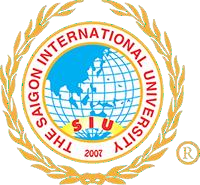
\includegraphics[height=1.8cm]{image/logo.png}\\[0.3cm]

\vspace{0.8cm}
{\fontsize{18}{22}\selectfont\bfseries BÀI ĐỒ ÁN CUỐI KỲ}\\[1.2cm]

{\fontsize{14}{18}\selectfont\bfseries HỌC PHẦN:\quad \hocphan}\\[1cm]

{\fontsize{14}{18}\selectfont\bfseries TÊN ĐỒ ÁN:}\\[0.3cm]
{\fontsize{14}{18}\selectfont\bfseries \tenduan}\\[1.5cm]

\begin{minipage}[t]{0.85\textwidth}
\fontsize{13}{17}\selectfont
\bfseries Giảng viên giảng dạy:\quad \giangvien\\[0.4cm]
\bfseries Học viên thực hiện:\quad \hocvien\\[0.4cm]
\bfseries Mã học viên:\quad \mahocvien\\[0.4cm]
\bfseries Lớp:\quad \lop \hspace{2cm} \bfseries Mã số lớp:\quad \malop\\[1.2cm]
\end{minipage}

\vfill
{\fontsize{13}{17}\selectfont\itshape TP. Hồ Chí Minh, tháng \thangnam}\\[0.6cm]
\end{center}

%==============================================================================
% BÌA 2 (trang 2 - theo mẫu BIA DO AN CUOI MON MCS.docx)
%==============================================================================
\newpage
\thispagestyle{empty}
{\setlength{\fboxrule}{4.5pt}\setlength{\fboxsep}{12pt}%
\noindent\fbox{\begin{minipage}{\dimexpr\textwidth-2\fboxsep-2\fboxrule}
\begin{center}
\vspace*{0.3cm}
{\fontsize{14}{18}\selectfont\bfseries BỘ GIÁO DỤC VÀ ĐÀO TẠO}\\[0.5cm]
{\fontsize{14}{18}\selectfont\bfseries TRƯỜNG ĐẠI HỌC TƯ THỤC QUỐC TẾ SÀI GÒN}\\[0.8cm]
{\fontsize{14}{18}\selectfont\bfseries *********}\\[1cm]

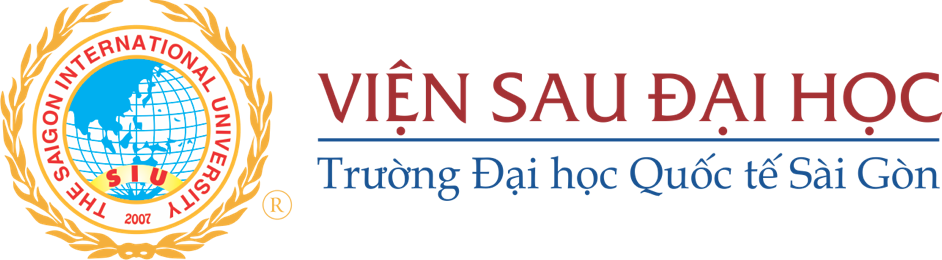
\includegraphics[width=11cm]{image/full-name-and-logo.png}\\[0.7cm]

{\fontsize{18}{22}\selectfont\bfseries BÀI CUỐI KỲ}\\[1.2cm]

\begin{tabular}{l l}
{\fontsize{14}{18}\selectfont\bfseries Ngành:} & \nganh \\[0.3cm]
{\fontsize{14}{18}\selectfont\bfseries Mã ngành:} & \manganh \\[0.3cm]
{\fontsize{14}{18}\selectfont\bfseries Mã lớp:} & \malop \\[0.3cm]
\end{tabular}

\end{center}
\begin{flushleft}
{\fontsize{14}{18}\selectfont\bfseries \uline{Nội dung nghiên cứu:}}\\[0.3cm]
\hspace{1cm}\noidungnghiencuu
\end{flushleft}
\vspace{1.2cm}

\begin{center}
\vfill
{\fontsize{13}{17}\selectfont\itshape TP. Hồ Chí Minh, tháng \thangnam}\\[0.8cm]
\end{center}

\end{minipage}}}

\begin{center}
  % Bảng chấm điểm
\begin{tabular}{|p{2.5cm}|p{3cm}|p{5cm}|p{3.5cm}|}
\hline
\multicolumn{2}{|c|}{\textbf{Điểm}} 
& \multicolumn{1}{c|}{\textbf{Nhận xét}} 
& \multicolumn{1}{c|}{\textbf{Giảng viên ký}} \\
\cline{1-2}
\textbf{Bằng số} & \textbf{Bằng chữ} & & \\
\hline
&  &  &  \\[2.5cm]
\hline
\end{tabular}
\end{center}

\newpage
\tableofcontents
\newpage
\setcounter{page}{1}

%==============================================================================
\section*{Mở đầu}
\addcontentsline{toc}{section}{\numberline{}Mở đầu}
%==============================================================================

Trong lịch sử tư tưởng nhân loại, sự ra đời của triết học đánh dấu một bước chuyển quan trọng trong cách con người nhận thức và giải thích thế giới. Nếu trong giai đoạn đầu của lịch sử, các hiện tượng tự nhiên và xã hội chủ yếu được giải thích thông qua thần thoại, tôn giáo và các niềm tin siêu nhiên, thì từ khoảng thiên niên kỷ I trước Công nguyên, ở nhiều nền văn minh lớn đã xuất hiện một xu hướng tư duy mới: giải thích thế giới bằng những nguyên lý mang tính lý tính và tự nhiên. Trong bối cảnh đó, chủ nghĩa duy vật cổ đại hình thành như một trong những khuynh hướng triết học sớm nhất nhằm khẳng định rằng bản chất của thế giới là vật chất và các hiện tượng tự nhiên có thể được lý giải bằng chính những quy luật nội tại của tự nhiên, thay vì dựa vào các lực lượng siêu nhiên.

Chủ nghĩa duy vật cổ đại xuất hiện ở nhiều trung tâm văn minh khác nhau, tiêu biểu nhất là trong triết học Hy Lạp cổ đại và triết học Trung Hoa cổ đại. Ở Hy Lạp, các nhà triết học tiền Socrates đã đặt ra câu hỏi về \emph{bản nguyên} (\emph{archê}) của thế giới và tìm kiếm những yếu tố vật chất cơ bản cấu thành nên mọi sự vật. Những quan niệm như nước của Thales, \emph{apeiron} của Anaximander, không khí của Anaximenes, hay đặc biệt là thuyết nguyên tử của Democritus đã thể hiện nỗ lực giải thích cấu trúc của vũ trụ trên cơ sở vật chất. Trong khi đó, ở Trung Hoa cổ đại, nhiều tư tưởng triết học cũng thể hiện những yếu tố duy vật rõ rệt, đặc biệt là quan niệm về \emph{khí} như một bản nguyên vật chất của vạn vật, cùng với học thuyết âm dương và ngũ hành nhằm giải thích sự vận động và biến đổi của tự nhiên.

Mặc dù được hình thành trong những bối cảnh văn hóa và lịch sử khác nhau, các quan niệm duy vật cổ đại đều có chung một đặc điểm quan trọng: chúng đánh dấu sự chuyển biến từ cách lý giải thế giới dựa trên thần thoại sang cách tiếp cận dựa trên tư duy lý tính. Nhờ đó, chủ nghĩa duy vật cổ đại đã góp phần đặt nền móng cho sự phát triển của tư duy khoa học và triết học sau này. Những nỗ lực tìm kiếm bản chất vật chất của thế giới, dù còn mang tính trực quan và sơ khai, đã mở ra một hướng tiếp cận mới đối với việc nghiên cứu tự nhiên, trong đó các hiện tượng được giải thích bằng những nguyên nhân nội tại thay vì các lực lượng siêu nhiên.

Tuy nhiên, bên cạnh những đóng góp quan trọng, chủ nghĩa duy vật cổ đại cũng mang những giới hạn lịch sử nhất định. Do điều kiện khoa học còn sơ khai và phương pháp nhận thức còn hạn chế, nhiều quan niệm về vật chất và cấu trúc của thế giới vẫn mang tính trực quan, cảm tính hoặc cơ học. Các nhà triết học cổ đại thường dựa chủ yếu vào quan sát và suy luận triết học, trong khi thiếu cơ sở thực nghiệm khoa học để kiểm chứng các giả thuyết của mình. Vì vậy, mặc dù chứa đựng những yếu tố hợp lý và tiến bộ, chủ nghĩa duy vật cổ đại vẫn chưa thể phát triển thành một hệ thống triết học hoàn chỉnh về mặt khoa học.

Từ góc độ lịch sử triết học, việc nghiên cứu chủ nghĩa duy vật cổ đại có ý nghĩa quan trọng không chỉ trong việc hiểu rõ nguồn gốc của tư duy duy vật, mà còn giúp làm sáng tỏ quá trình phát triển của tư tưởng triết học nói chung. Thông qua việc phân tích những quan niệm về bản nguyên vật chất, cấu trúc của thế giới và sự vận động của tự nhiên trong các hệ thống triết học cổ đại, có thể thấy được những bước tiến quan trọng trong quá trình hình thành thế giới quan khoa học của nhân loại. Đồng thời, việc nhận diện những hạn chế lịch sử của các quan niệm này cũng giúp hiểu rõ hơn những điều kiện cần thiết cho sự phát triển của triết học và khoa học trong các giai đoạn sau.

Trên cơ sở đó, bài luận này hướng tới việc phân tích sự hình thành và đặc điểm tư duy của chủ nghĩa duy vật cổ đại, đồng thời làm rõ giá trị triết học cũng như những giới hạn lịch sử của nó trong tiến trình phát triển của tư tưởng nhân loại. Cụ thể, bài viết tập trung trả lời ba câu hỏi nghiên cứu chính: (1) chủ nghĩa duy vật cổ đại hình thành trong bối cảnh lịch sử và tri thức như thế nào; (2) những quan niệm triết học cơ bản của nó về bản nguyên vật chất và cấu trúc của thế giới là gì; và (3) những đóng góp cũng như hạn chế của chủ nghĩa duy vật cổ đại đối với lịch sử triết học là gì.

Để giải quyết các vấn đề trên, bài luận sử dụng phương pháp phân tích triết học kết hợp với phương pháp lịch sử và so sánh. Thông qua việc xem xét các tư tưởng duy vật tiêu biểu trong triết học Hy Lạp và Trung Hoa cổ đại, bài viết không chỉ làm rõ nội dung của các quan niệm này mà còn chỉ ra những điểm tương đồng và khác biệt trong cách tiếp cận vấn đề bản nguyên của thế giới.

Về cấu trúc, bài luận được chia thành hai chương chính. Chương thứ nhất tập trung phân tích bối cảnh hình thành và cấu trúc tư duy của chủ nghĩa duy vật cổ đại, bao gồm các hình thức biểu hiện tiêu biểu trong triết học Hy Lạp và Trung Hoa. Chương thứ hai sẽ đánh giá giá trị triết học cũng như những giới hạn lịch sử của các quan niệm duy vật cổ đại, đồng thời xem xét ảnh hưởng của chúng đối với sự phát triển của triết học và thế giới quan khoa học trong các giai đoạn sau. Thông qua đó, bài luận hướng tới việc làm rõ vị trí và ý nghĩa của chủ nghĩa duy vật cổ đại trong lịch sử tư tưởng nhân loại.

%==============================================================================
\section{Sự hình thành và cấu trúc tư duy của chủ nghĩa duy vật cổ đại}
%==============================================================================

\subsection{Bối cảnh lịch sử -- tri thức của sự ra đời chủ nghĩa duy vật cổ đại}

Sự ra đời của chủ nghĩa duy vật cổ đại không phải là một hiện tượng ngẫu nhiên trong lịch sử tư tưởng, mà là kết quả của những biến đổi sâu sắc trong đời sống kinh tế, xã hội và nhận thức của con người ở các nền văn minh cổ đại. Từ khoảng thiên niên kỷ I trước Công nguyên, nhiều trung tâm văn minh lớn như Hy Lạp và Trung Hoa đã bước vào một giai đoạn phát triển mới, trong đó các hình thức tổ chức xã hội, hoạt động kinh tế và giao lưu văn hóa ngày càng trở nên phức tạp. Chính những điều kiện này đã tạo ra nhu cầu giải thích thế giới một cách hợp lý hơn, góp phần thúc đẩy sự hình thành của tư duy triết học nói chung và các quan niệm duy vật nói riêng.

Trước khi triết học xuất hiện, cách con người lý giải thế giới chủ yếu dựa vào thần thoại và tôn giáo. Trong các hệ thống thần thoại cổ đại, tự nhiên thường được nhân cách hóa thành các vị thần có ý chí và quyền năng siêu nhiên, chi phối sự vận động của vũ trụ cũng như đời sống con người. Những hiện tượng như sấm sét, mưa gió, mùa màng hay thiên tai được xem là biểu hiện của quyền lực thần linh. Mặc dù thần thoại có vai trò quan trọng trong việc hình thành thế giới quan ban đầu của con người, song cách giải thích này mang tính biểu tượng và thiếu tính hệ thống lý luận.

Sự phát triển của đời sống xã hội đã dần làm xuất hiện những nhu cầu nhận thức mới. Khi hoạt động sản xuất, thương mại và hàng hải ngày càng mở rộng, con người cần hiểu rõ hơn các quy luật của tự nhiên để phục vụ cho đời sống thực tiễn. Những kinh nghiệm tích lũy trong các lĩnh vực như thiên văn học, toán học, nông nghiệp hay y học đã góp phần làm phong phú tri thức của con người về thế giới tự nhiên. Từ đó, một xu hướng tư duy mới dần hình thành: thay vì giải thích các hiện tượng bằng ý chí của thần linh, con người bắt đầu tìm kiếm những nguyên nhân tự nhiên và khách quan nằm trong chính bản thân thế giới vật chất.

Trong bối cảnh đó, triết học cổ đại ra đời như một hình thức tư duy lý luận nhằm khái quát và hệ thống hóa những tri thức về thế giới. Một trong những vấn đề trung tâm mà các nhà triết học cổ đại quan tâm là câu hỏi về bản nguyên của vũ trụ: thế giới được cấu thành từ cái gì và vì sao nó tồn tại trong trạng thái vận động và biến đổi không ngừng. Việc đặt ra câu hỏi này cho thấy một bước tiến quan trọng trong nhận thức, bởi nó hướng tới việc tìm kiếm những nguyên lý chung của tự nhiên thay vì chỉ mô tả các hiện tượng riêng lẻ.

Ở Hy Lạp cổ đại, sự phát triển của các thành bang, đặc biệt là các trung tâm thương mại ven biển, đã tạo điều kiện thuận lợi cho sự giao lưu văn hóa và tri thức giữa nhiều nền văn minh khác nhau. Những tiếp xúc với tri thức của Ai Cập và Lưỡng Hà đã góp phần thúc đẩy sự phát triển của khoa học và triết học Hy Lạp. Trong môi trường trí tuệ tương đối cởi mở này, các nhà triết học tiền Socrates bắt đầu đặt ra những câu hỏi mang tính nền tảng về cấu trúc của thế giới tự nhiên. Thay vì viện dẫn các câu chuyện thần thoại, họ tìm cách giải thích sự hình thành và vận động của vũ trụ bằng những yếu tố vật chất cơ bản. Đây chính là bước khởi đầu của tư duy duy vật trong triết học phương Tây.

Ở Trung Hoa cổ đại, những biến động xã hội sâu sắc trong thời kỳ Xuân Thu -- Chiến Quốc cũng đã thúc đẩy sự phát triển mạnh mẽ của tư tưởng triết học. Trong bối cảnh trật tự xã hội truyền thống bị lung lay, nhiều học phái triết học đã xuất hiện nhằm tìm kiếm những nguyên lý giải thích tự nhiên và xã hội. Bên cạnh các hệ thống tư tưởng mang tính đạo đức -- chính trị như Nho gia hay Pháp gia, nhiều quan niệm về tự nhiên cũng được hình thành, đặc biệt là học thuyết về khí, âm dương và ngũ hành. Những quan niệm này, dù chưa phát triển thành một hệ thống duy vật hoàn chỉnh theo nghĩa chặt chẽ, nhưng đã thể hiện rõ xu hướng giải thích thế giới bằng các yếu tố vật chất và các quy luật vận động nội tại của tự nhiên.

Nhìn chung, sự ra đời của chủ nghĩa duy vật cổ đại gắn liền với quá trình chuyển biến từ tư duy thần thoại sang tư duy lý tính trong lịch sử nhận thức của nhân loại. Các nhà triết học cổ đại đã cố gắng tìm kiếm những nguyên lý vật chất cơ bản nhằm giải thích sự tồn tại và vận động của vũ trụ. Mặc dù những quan niệm này còn mang tính sơ khai và chịu nhiều hạn chế do điều kiện khoa học thời bấy giờ, nhưng chúng đã mở ra một hướng tiếp cận mới đối với việc nghiên cứu thế giới tự nhiên. Chính từ nền tảng đó, các hình thức tư duy duy vật khác nhau đã dần được hình thành và phát triển trong các hệ thống triết học cổ đại.

\subsection{Các hình thức chủ nghĩa duy vật trong triết học Hy Lạp cổ đại}

Triết học Hy Lạp cổ đại được xem là một trong những cái nôi quan trọng của tư duy triết học phương Tây. Trong quá trình hình thành và phát triển của nó, nhiều nhà tư tưởng đã cố gắng tìm kiếm bản nguyên của thế giới thông qua các yếu tố vật chất cụ thể. Những nỗ lực này đã đặt nền móng cho sự xuất hiện của chủ nghĩa duy vật trong triết học phương Tây. Mặc dù các quan niệm duy vật trong giai đoạn này còn mang tính trực quan và chưa hình thành một hệ thống lý luận hoàn chỉnh, song chúng đã thể hiện rõ xu hướng giải thích thế giới bằng những nguyên nhân tự nhiên thay vì dựa vào các lực lượng siêu nhiên.

\subsubsection{Trường phái Miletus và sự tìm kiếm bản nguyên vật chất}

Những biểu hiện sớm nhất của tư duy duy vật trong triết học Hy Lạp cổ đại xuất hiện trong các triết gia thuộc trường phái Miletus vào khoảng thế kỷ VI trước Công nguyên. Các nhà tư tưởng của trường phái này tập trung vào việc tìm kiếm \emph{archê} -- bản nguyên cơ bản của vũ trụ, tức yếu tố đầu tiên từ đó mọi sự vật được hình thành và phát triển.

Thales, người thường được xem là nhà triết học đầu tiên của Hy Lạp cổ đại, cho rằng bản nguyên của mọi sự vật là nước. Theo ông, nước tồn tại trong nhiều trạng thái khác nhau và đóng vai trò thiết yếu đối với sự sống cũng như sự hình thành của thế giới tự nhiên. Mặc dù quan niệm này mang tính đơn giản và trực quan, song nó có ý nghĩa quan trọng ở chỗ đã tìm cách giải thích sự tồn tại của thế giới bằng một yếu tố vật chất cụ thể, thay vì viện dẫn các yếu tố thần thoại.

Tiếp nối tư tưởng của Thales, Anaximander cho rằng bản nguyên của thế giới không phải là một yếu tố vật chất cụ thể như nước, mà là một thực thể vô định và vô hạn mà ông gọi là \emph{apeiron}. Theo quan niệm của ông, từ \emph{apeiron} đã phát sinh ra các yếu tố đối lập như nóng -- lạnh, khô -- ẩm, và chính sự tương tác giữa các yếu tố này tạo nên sự đa dạng của thế giới tự nhiên. Tư tưởng của Anaximander thể hiện một bước tiến trong tư duy triết học, bởi ông đã cố gắng tìm kiếm một nguyên lý chung mang tính trừu tượng hơn để giải thích nguồn gốc của vũ trụ.

Anaximenes, một triết gia khác của trường phái Miletus, lại cho rằng không khí là bản nguyên của thế giới. Theo ông, mọi sự vật đều được hình thành từ không khí thông qua các quá trình cô đặc và loãng ra. Chẳng hạn, khi không khí bị cô đặc sẽ trở thành gió, mây, nước, đất và đá; ngược lại, khi loãng ra sẽ trở thành lửa. Quan niệm này cho thấy nỗ lực giải thích sự đa dạng của các sự vật trong tự nhiên thông qua sự biến đổi của một yếu tố vật chất cơ bản.

Mặc dù mỗi nhà triết học của trường phái Miletus đưa ra một bản nguyên khác nhau, điểm chung trong tư tưởng của họ là đều cố gắng tìm kiếm một nguyên lý vật chất có khả năng giải thích nguồn gốc và cấu trúc của thế giới. Chính sự tìm kiếm này đã đánh dấu bước chuyển quan trọng từ tư duy thần thoại sang tư duy triết học mang tính lý tính.

\subsubsection{Thuyết nguyên tử và quan niệm về cấu trúc của thế giới}

Một trong những hình thức phát triển quan trọng nhất của chủ nghĩa duy vật trong triết học Hy Lạp cổ đại là thuyết nguyên tử, gắn liền với tên tuổi của Leucippus và Democritus vào thế kỷ V trước Công nguyên. Theo học thuyết này, thế giới được cấu thành từ vô số các hạt vật chất cực nhỏ gọi là nguyên tử (\emph{atomos}), tồn tại trong khoảng không gian trống rỗng gọi là chân không.

Các nguyên tử được cho là không thể chia nhỏ hơn, có tính vĩnh cửu và bất biến. Sự khác nhau giữa các sự vật trong thế giới không phải do bản chất khác nhau của các nguyên tử, mà do sự khác nhau về hình dạng, kích thước, vị trí và cách sắp xếp của chúng. Khi các nguyên tử kết hợp với nhau theo những cấu trúc khác nhau, chúng tạo nên các vật thể khác nhau trong tự nhiên. Ngược lại, khi các cấu trúc này bị phá vỡ, các sự vật cũng tan rã.

Thuyết nguyên tử của Democritus thể hiện một bước tiến quan trọng trong tư duy duy vật cổ đại, bởi nó đã đưa ra một mô hình giải thích tương đối nhất quán về cấu trúc của thế giới vật chất. Theo quan niệm này, mọi hiện tượng tự nhiên đều có thể được giải thích thông qua sự vận động và tương tác của các nguyên tử trong chân không, mà không cần đến sự can thiệp của các lực lượng siêu nhiên.

\subsubsection{Sự phát triển của chủ nghĩa duy vật trong triết học Epicurus}

Đến thế kỷ IV--III trước Công nguyên, Epicurus đã tiếp thu và phát triển thuyết nguyên tử của Democritus, đồng thời đưa vào đó một số điều chỉnh quan trọng. Theo Epicurus, các nguyên tử vẫn là những hạt vật chất cơ bản cấu thành thế giới, nhưng trong quá trình vận động của chúng tồn tại một yếu tố lệch hướng nhỏ, thường được gọi là sự ``lệch'' (\emph{clinamen}). Nhờ sự lệch này, các nguyên tử có thể va chạm và kết hợp với nhau để hình thành nên các sự vật trong thế giới.

Việc đưa yếu tố ngẫu nhiên vào trong thuyết nguyên tử có ý nghĩa quan trọng đối với triết học của Epicurus. Nó cho phép ông giải thích sự hình thành của thế giới mà không cần đến sự chi phối của các lực lượng tất định tuyệt đối, đồng thời mở ra khả năng lý giải về tự do của con người. Theo Epicurus, nếu mọi sự vật đều vận động theo những quy luật tất định hoàn toàn, thì con người sẽ không có khả năng tự do lựa chọn hành động của mình. Vì vậy, sự tồn tại của yếu tố ngẫu nhiên trong tự nhiên giúp tạo ra không gian cho tự do của ý chí.

Nhìn chung, các hình thức duy vật trong triết học Hy Lạp cổ đại đã thể hiện nỗ lực mạnh mẽ của các nhà tư tưởng trong việc tìm kiếm những nguyên lý vật chất cơ bản của thế giới. Từ việc xác định các yếu tố tự nhiên như nước hay không khí là bản nguyên của vũ trụ, đến việc xây dựng học thuyết nguyên tử nhằm giải thích cấu trúc của vật chất, các nhà triết học Hy Lạp cổ đại đã đặt những nền móng quan trọng cho sự phát triển của tư duy duy vật trong lịch sử triết học phương Tây. Mặc dù những quan niệm này còn mang tính sơ khai và chịu nhiều hạn chế do điều kiện khoa học của thời đại, nhưng chúng đã mở ra một cách tiếp cận mới đối với việc nghiên cứu thế giới tự nhiên, dựa trên các nguyên nhân vật chất và quy luật nội tại của tự nhiên.

\subsection{Các yếu tố duy vật trong triết học Trung Hoa cổ đại}

Bên cạnh triết học Hy Lạp cổ đại, trong lịch sử tư tưởng phương Đông cũng xuất hiện nhiều quan niệm mang tính duy vật nhằm giải thích cấu trúc và sự vận động của thế giới tự nhiên. Trong triết học Trung Hoa cổ đại, mặc dù các học thuyết thường gắn liền với những vấn đề đạo đức, chính trị và trật tự xã hội, song nhiều hệ thống tư tưởng vẫn chứa đựng những yếu tố duy vật đáng chú ý. Đặc biệt, các quan niệm về \emph{khí}, học thuyết \emph{âm dương} và \emph{ngũ hành}, cũng như tư tưởng của một số nhà triết học như Tuân Tử đã thể hiện xu hướng giải thích thế giới dựa trên các yếu tố vật chất và những quy luật vận động nội tại của tự nhiên.

\subsubsection{Quan niệm về khí như bản nguyên của thế giới}

Một trong những khái niệm trung tâm trong nhiều hệ thống tư tưởng Trung Hoa cổ đại là khái niệm \emph{khí}. Theo quan niệm này, khí được xem là yếu tố vật chất cơ bản cấu thành nên mọi sự vật và hiện tượng trong vũ trụ. Khí không phải là một thực thể tĩnh tại, mà luôn tồn tại trong trạng thái vận động và biến đổi, từ đó tạo nên sự đa dạng của thế giới tự nhiên.

Trong nhiều văn bản triết học cổ đại, khí được mô tả như một dạng vật chất tinh vi và phổ biến khắp vũ trụ. Tất cả các sự vật, từ những hiện tượng tự nhiên như trời, đất, núi, sông cho đến con người và các sinh vật sống, đều được cho là hình thành từ sự kết hợp và biến đổi của khí. Khi khí tụ lại thì hình thành các vật thể cụ thể; khi khí tán ra thì các sự vật tan rã và trở về trạng thái ban đầu.

Quan niệm về khí thể hiện một cách nhìn mang tính duy vật ở chỗ nó coi thế giới là một chỉnh thể vật chất thống nhất. Mọi hiện tượng đều được giải thích thông qua sự vận động và biến đổi của khí, chứ không phải thông qua sự can thiệp của các lực lượng siêu nhiên. Nhờ đó, khái niệm này đã góp phần hình thành một cách tiếp cận tự nhiên đối với việc lý giải vũ trụ.

\subsubsection{Học thuyết âm dương và ngũ hành}

Bên cạnh quan niệm về khí, học thuyết âm dương và ngũ hành cũng đóng vai trò quan trọng trong việc giải thích cấu trúc và sự vận động của thế giới trong triết học Trung Hoa cổ đại. Theo học thuyết âm dương, mọi sự vật và hiện tượng trong vũ trụ đều chứa đựng hai mặt đối lập nhưng bổ sung cho nhau là âm và dương. Hai yếu tố này không tồn tại tách biệt mà luôn vận động, chuyển hóa và tương tác với nhau, tạo nên sự biến đổi không ngừng của thế giới tự nhiên.

Âm thường được gắn với những đặc tính như tĩnh, tối, lạnh và mềm; trong khi dương gắn với những đặc tính như động, sáng, nóng và cứng. Tuy nhiên, âm và dương không phải là những thực thể độc lập, mà chỉ là hai mặt của cùng một quá trình vận động của tự nhiên. Sự cân bằng và chuyển hóa giữa âm và dương được xem là nguyên lý cơ bản chi phối sự tồn tại và phát triển của vạn vật.

Bổ sung cho học thuyết âm dương là học thuyết ngũ hành, trong đó thế giới được cho là cấu thành từ năm yếu tố cơ bản: kim, mộc, thủy, hỏa và thổ. Các yếu tố này không chỉ tồn tại riêng lẻ mà còn có mối quan hệ tương sinh và tương khắc với nhau. Chính sự tương tác giữa các yếu tố này được xem là nguyên nhân của những biến đổi và chu trình vận động trong tự nhiên.

Mặc dù học thuyết âm dương và ngũ hành mang nhiều yếu tố biểu tượng và chưa có cơ sở khoa học theo nghĩa hiện đại, nhưng chúng đã thể hiện một nỗ lực quan trọng nhằm giải thích các hiện tượng tự nhiên bằng những quy luật nội tại của thế giới vật chất. Thay vì dựa vào ý chí của thần linh, các học thuyết này tìm cách mô tả những nguyên lý phổ quát chi phối sự vận động của vũ trụ.

\subsubsection{Tư tưởng duy vật trong triết học Tuân Tử}

Trong số các nhà tư tưởng Trung Hoa cổ đại, Tuân Tử được xem là một trong những người thể hiện rõ nhất xu hướng duy vật trong cách nhìn về tự nhiên. Khác với nhiều quan niệm truyền thống cho rằng thiên nhiên có ý chí hay mục đích riêng, Tuân Tử cho rằng trời và đất vận hành theo những quy luật khách quan, không phụ thuộc vào mong muốn của con người.

Theo Tuân Tử, các hiện tượng tự nhiên như sự thay đổi của mùa, sự vận động của mặt trời và mặt trăng hay sự sinh trưởng của vạn vật đều diễn ra theo những quy luật nhất định của tự nhiên. Những quy luật này không chịu sự chi phối của các lực lượng siêu nhiên hay ý chí thần linh. Vì vậy, con người không nên tìm cách cầu xin hoặc dựa vào các yếu tố thần bí để thay đổi tự nhiên, mà cần hiểu rõ các quy luật của nó để có thể thích ứng và sử dụng chúng một cách hợp lý.

Quan điểm này thể hiện rõ tinh thần duy vật trong triết học của Tuân Tử. Ông nhấn mạnh rằng thiên nhiên tồn tại độc lập với con người và vận hành theo những quy luật khách quan. Nhiệm vụ của con người không phải là thay đổi các quy luật đó, mà là nhận thức và vận dụng chúng trong đời sống thực tiễn.

Nhìn chung, các quan niệm về khí, âm dương -- ngũ hành và tư tưởng của Tuân Tử đã góp phần hình thành những yếu tố duy vật quan trọng trong triết học Trung Hoa cổ đại. Mặc dù các hệ thống tư tưởng này chưa phát triển thành một chủ nghĩa duy vật hoàn chỉnh theo nghĩa lý luận chặt chẽ, nhưng chúng đã thể hiện rõ xu hướng giải thích thế giới bằng các yếu tố vật chất và các quy luật vận động nội tại của tự nhiên. Điều này cho thấy rằng tư duy duy vật không chỉ xuất hiện trong triết học phương Tây mà còn có những biểu hiện đáng kể trong truyền thống triết học phương Đông.

\subsection{Hai mô hình bản thể luận của chủ nghĩa duy vật cổ đại}

Từ việc khảo sát các tư tưởng duy vật trong triết học Hy Lạp và Trung Hoa cổ đại, có thể nhận thấy rằng mặc dù cùng hướng tới việc giải thích thế giới trên cơ sở vật chất, các hệ thống triết học này đã hình thành những cách tiếp cận khác nhau đối với bản chất và cấu trúc của thực tại. Những cách tiếp cận đó có thể được khái quát thành hai mô hình bản thể luận cơ bản: mô hình vật chất rời rạc và mô hình vật chất liên tục. Hai mô hình này phản ánh những cách hiểu khác nhau về bản nguyên của thế giới cũng như về cách thức mà các sự vật hình thành và biến đổi trong tự nhiên.

\subsubsection{Mô hình vật chất rời rạc}

Mô hình vật chất rời rạc được thể hiện rõ nét nhất trong thuyết nguyên tử của các nhà triết học Hy Lạp cổ đại, đặc biệt là trong tư tưởng của Leucippus và Democritus. Theo quan niệm này, thế giới được cấu thành từ vô số những hạt vật chất cực nhỏ gọi là nguyên tử. Các nguyên tử được cho là không thể phân chia, tồn tại vĩnh viễn và không thay đổi về bản chất. Chúng khác nhau về hình dạng, kích thước và vị trí trong không gian, và chính sự khác nhau này tạo nên sự đa dạng của các sự vật trong thế giới.

Trong mô hình này, thế giới được hiểu như một tập hợp các đơn vị vật chất độc lập vận động trong khoảng không gian trống rỗng. Các hiện tượng tự nhiên được giải thích thông qua sự chuyển động, va chạm và kết hợp của các nguyên tử. Khi các nguyên tử kết hợp theo những cấu trúc khác nhau, chúng tạo thành các vật thể cụ thể; khi các cấu trúc này bị phá vỡ, các vật thể cũng tan rã và trở về trạng thái ban đầu của các nguyên tử.

Mô hình vật chất rời rạc có ý nghĩa quan trọng trong lịch sử tư tưởng bởi nó đã đưa ra một cách giải thích tương đối nhất quán về cấu trúc của thế giới vật chất. Thay vì xem các sự vật là những thực thể độc lập được tạo ra bởi các lực lượng siêu nhiên, thuyết nguyên tử cho rằng tất cả các hiện tượng đều có thể được giải thích bằng sự vận động của các yếu tố vật chất cơ bản. Nhờ đó, mô hình này đã đặt nền tảng cho nhiều quan niệm khoa học về cấu trúc của vật chất trong các giai đoạn sau.

\subsubsection{Mô hình vật chất liên tục}

Khác với mô hình vật chất rời rạc của thuyết nguyên tử, trong nhiều hệ thống triết học phương Đông -- đặc biệt là trong triết học Trung Hoa cổ đại -- thế giới thường được hiểu theo mô hình vật chất liên tục. Theo cách nhìn này, bản nguyên của vũ trụ không phải là những đơn vị vật chất tách rời nhau, mà là một dạng vật chất thống nhất và liên tục, thường được biểu hiện thông qua khái niệm khí.

Trong quan niệm này, khí tồn tại khắp nơi trong vũ trụ và luôn vận động, biến đổi không ngừng. Các sự vật cụ thể được hình thành khi khí tụ lại trong những hình thức nhất định; khi khí tán ra, các sự vật lại trở về trạng thái ban đầu. Do đó, sự khác biệt giữa các sự vật không phải là kết quả của những yếu tố vật chất hoàn toàn khác nhau, mà chủ yếu là do sự khác nhau về trạng thái, mức độ tập trung hoặc sự vận động của cùng một bản nguyên vật chất.

Mô hình vật chất liên tục thường gắn liền với quan niệm về sự vận động và biến đổi không ngừng của tự nhiên. Thông qua các học thuyết như âm dương và ngũ hành, triết học Trung Hoa cổ đại đã nhấn mạnh rằng các yếu tố trong tự nhiên luôn tương tác và chuyển hóa lẫn nhau. Sự vận động này tạo nên quá trình biến đổi liên tục của vạn vật trong vũ trụ.

\subsubsection{So sánh hai mô hình bản thể luận}

Mặc dù có những điểm khác biệt đáng kể, hai mô hình bản thể luận trên đều thể hiện một điểm chung quan trọng: chúng đều khẳng định tính vật chất của thế giới và cố gắng giải thích các hiện tượng tự nhiên bằng những nguyên lý nội tại của tự nhiên. Cả hai cách tiếp cận đều tìm cách loại bỏ vai trò của các lực lượng siêu nhiên trong việc giải thích sự tồn tại và vận động của vũ trụ.

Tuy nhiên, giữa hai mô hình vẫn tồn tại những khác biệt cơ bản. Mô hình vật chất rời rạc nhấn mạnh đến cấu trúc của vật chất như một tập hợp các đơn vị riêng biệt, từ đó giải thích các hiện tượng tự nhiên thông qua sự vận động và tương tác cơ học giữa các đơn vị này. Trong khi đó, mô hình vật chất liên tục lại xem thế giới như một chỉnh thể thống nhất, trong đó các sự vật chỉ là những trạng thái khác nhau của cùng một bản nguyên vật chất.

Sự khác biệt này phản ánh những định hướng triết học khác nhau trong cách tiếp cận vấn đề bản nguyên của thế giới. Triết học Hy Lạp cổ đại thường có xu hướng phân tích và tìm kiếm các yếu tố cấu thành cơ bản của thực tại, trong khi triết học Trung Hoa cổ đại lại nhấn mạnh tính tổng thể và sự vận động liên tục của vũ trụ. Tuy vậy, cả hai cách tiếp cận đều đóng góp quan trọng vào sự hình thành của tư duy duy vật trong lịch sử triết học.

Nhìn chung, hai mô hình bản thể luận này cho thấy sự phong phú và đa dạng của các quan niệm duy vật trong thời cổ đại. Chúng không chỉ phản ánh những nỗ lực ban đầu của con người trong việc hiểu bản chất của thế giới, mà còn đặt nền móng cho nhiều cuộc tranh luận triết học về cấu trúc và bản chất của vật chất trong các giai đoạn sau của lịch sử tư tưởng.

%==============================================================================
\section{Giá trị triết học và giới hạn lịch sử của chủ nghĩa duy vật cổ đại}
%==============================================================================

\subsection{Giá trị triết học của chủ nghĩa duy vật cổ đại}

Chủ nghĩa duy vật cổ đại giữ một vị trí quan trọng trong lịch sử phát triển của tư tưởng triết học. Mặc dù được hình thành trong những điều kiện khoa học và nhận thức còn hạn chế, các quan niệm duy vật cổ đại đã góp phần đặt nền móng cho cách tiếp cận lý tính trong việc giải thích thế giới. Thông qua việc khẳng định bản chất vật chất của vũ trụ và tìm kiếm các nguyên nhân tự nhiên của các hiện tượng, chủ nghĩa duy vật cổ đại đã mở ra một hướng phát triển mới cho tư duy triết học và khoa học.

\subsubsection{Bước chuyển từ tư duy thần thoại sang giải thích lý tính về thế giới}

Một trong những giá trị quan trọng nhất của chủ nghĩa duy vật cổ đại là góp phần thúc đẩy quá trình chuyển biến từ tư duy thần thoại sang tư duy lý tính trong lịch sử nhận thức của nhân loại. Trong giai đoạn trước khi triết học xuất hiện, con người thường giải thích các hiện tượng tự nhiên thông qua các câu chuyện thần thoại hoặc niềm tin vào quyền lực của các vị thần. Những cách giải thích này tuy có ý nghĩa về mặt văn hóa và tinh thần, nhưng thường mang tính biểu tượng và thiếu cơ sở lý luận.

Sự xuất hiện của các nhà triết học duy vật cổ đại đã tạo ra một cách tiếp cận khác đối với việc lý giải thế giới. Thay vì viện dẫn các lực lượng siêu nhiên, họ tìm cách xác định những yếu tố vật chất cơ bản và các quy luật tự nhiên chi phối sự vận động của vũ trụ. Việc đặt ra câu hỏi về bản nguyên của thế giới, cũng như nỗ lực tìm kiếm những nguyên lý chung để giải thích các hiện tượng tự nhiên, đã đánh dấu sự ra đời của tư duy triết học theo nghĩa chặt chẽ.

Chính sự chuyển biến này đã góp phần hình thành một thái độ nhận thức mới, trong đó thế giới được xem là một hệ thống có thể được hiểu và giải thích thông qua lý trí của con người. Đây là bước tiến quan trọng trong lịch sử trí tuệ, bởi nó mở đường cho sự phát triển của khoa học và triết học trong các giai đoạn sau.

\subsubsection{Khẳng định tính vật chất của thế giới}

Một đóng góp quan trọng khác của chủ nghĩa duy vật cổ đại là việc khẳng định rằng thế giới có bản chất vật chất và tồn tại độc lập với ý thức của con người. Các nhà triết học duy vật cổ đại, dù xuất phát từ những cách tiếp cận khác nhau, đều cố gắng giải thích sự hình thành và vận động của vũ trụ dựa trên các yếu tố vật chất.

Chẳng hạn, trong triết học Hy Lạp cổ đại, các nhà tư tưởng thuộc trường phái Miletus đã tìm kiếm bản nguyên của thế giới trong các yếu tố tự nhiên như nước hoặc không khí. Sau đó, thuyết nguyên tử đã phát triển quan niệm này theo hướng cho rằng thế giới được cấu thành từ những hạt vật chất cơ bản tồn tại trong chân không. Trong triết học Trung Hoa cổ đại, quan niệm về khí cũng thể hiện cách nhìn coi vật chất là nền tảng của mọi sự vật và hiện tượng trong vũ trụ.

Những quan niệm này, mặc dù còn mang tính trực quan và chưa có cơ sở khoa học vững chắc theo tiêu chuẩn hiện đại, nhưng đã đặt nền tảng cho một thế giới quan duy vật. Việc khẳng định rằng các hiện tượng tự nhiên có thể được giải thích thông qua các yếu tố vật chất và các quy luật tự nhiên đã góp phần hình thành cơ sở lý luận cho sự phát triển của khoa học tự nhiên trong lịch sử.

\subsubsection{Những yếu tố biện chứng tự phát trong tư duy cổ đại}

Ngoài việc khẳng định tính vật chất của thế giới, nhiều quan niệm duy vật cổ đại còn chứa đựng những yếu tố biện chứng tự phát trong cách nhìn về sự vận động và biến đổi của tự nhiên. Các nhà triết học cổ đại đã nhận thấy rằng thế giới không phải là một thực thể tĩnh tại, mà luôn tồn tại trong trạng thái biến đổi và phát triển.

Trong triết học Hy Lạp cổ đại, thuyết nguyên tử đã giải thích sự hình thành và tan rã của các sự vật thông qua sự kết hợp và phân tách của các nguyên tử. Điều này cho thấy một cách hiểu sơ khai về quá trình vận động và biến đổi của vật chất. Tương tự, trong triết học Trung Hoa cổ đại, học thuyết âm dương nhấn mạnh sự tồn tại của các mặt đối lập trong tự nhiên và sự chuyển hóa lẫn nhau giữa chúng. Quan niệm này phản ánh một cách nhìn năng động về thế giới, trong đó sự vận động và biến đổi được xem là đặc điểm cơ bản của thực tại.

Những yếu tố biện chứng tự phát này cho thấy rằng các nhà triết học cổ đại đã bước đầu nhận thức được tính vận động, biến đổi và liên hệ của các sự vật trong thế giới. Mặc dù chưa phát triển thành một phương pháp biện chứng hoàn chỉnh, các quan niệm này đã góp phần chuẩn bị những tiền đề quan trọng cho sự hình thành của các hệ thống triết học biện chứng trong các giai đoạn sau của lịch sử tư tưởng.

Nhìn chung, chủ nghĩa duy vật cổ đại có giá trị to lớn trong việc đặt nền móng cho sự phát triển của tư duy triết học và khoa học. Thông qua việc khẳng định tính vật chất của thế giới, tìm kiếm các quy luật tự nhiên và nhận thức bước đầu về sự vận động của thực tại, các nhà triết học cổ đại đã mở ra một hướng tiếp cận mới đối với việc nghiên cứu vũ trụ và vị trí của con người trong thế giới. Mặc dù những quan niệm này còn mang nhiều hạn chế lịch sử, nhưng giá trị của chúng vẫn được ghi nhận như những bước khởi đầu quan trọng trong quá trình phát triển của tư tưởng triết học nhân loại.

\subsection{Những hạn chế lịch sử của chủ nghĩa duy vật cổ đại}

Mặc dù chủ nghĩa duy vật cổ đại có những đóng góp quan trọng đối với sự phát triển của tư duy triết học và khoa học, các quan niệm duy vật trong giai đoạn này vẫn mang những hạn chế nhất định do điều kiện lịch sử và trình độ nhận thức của thời đại. Những hạn chế này không làm giảm giá trị lịch sử của chủ nghĩa duy vật cổ đại, nhưng cho thấy rằng các quan niệm này mới chỉ là những bước khởi đầu trong quá trình phát triển lâu dài của tư tưởng duy vật.

\subsubsection{Tính trực quan và cảm tính trong quan niệm về vật chất}

Một trong những hạn chế cơ bản của chủ nghĩa duy vật cổ đại là tính trực quan và cảm tính trong cách hiểu về vật chất. Do khoa học tự nhiên thời cổ đại chưa phát triển, các nhà triết học thường dựa chủ yếu vào quan sát trực tiếp và suy luận triết học để hình thành các quan niệm của mình về cấu trúc của thế giới.

Vì vậy, nhiều nhà tư tưởng đã xác định bản nguyên của vũ trụ thông qua những yếu tố vật chất cụ thể và quen thuộc trong đời sống như nước, không khí hoặc lửa. Những quan niệm này phản ánh nỗ lực tìm kiếm một nền tảng vật chất cho thế giới, nhưng đồng thời cũng cho thấy sự hạn chế trong khả năng nhận thức về cấu trúc thực sự của vật chất. Ngay cả thuyết nguyên tử, mặc dù có ý nghĩa quan trọng trong lịch sử tư tưởng, cũng chủ yếu dựa trên suy luận triết học chứ chưa được chứng minh bằng các phương pháp khoa học thực nghiệm.

Tương tự, trong triết học Trung Hoa cổ đại, các khái niệm như khí hay các yếu tố trong học thuyết ngũ hành cũng mang tính khái quát trực quan về thế giới tự nhiên. Những quan niệm này thể hiện nỗ lực giải thích sự đa dạng của các hiện tượng tự nhiên, nhưng vẫn thiếu những cơ sở khoa học rõ ràng để kiểm chứng.

\subsubsection{Thiếu cơ sở khoa học thực nghiệm}

Một hạn chế quan trọng khác của chủ nghĩa duy vật cổ đại là sự thiếu vắng các phương pháp khoa học thực nghiệm. Trong thời cổ đại, khoa học tự nhiên chưa phát triển thành các ngành nghiên cứu độc lập với những phương pháp nghiên cứu chặt chẽ. Do đó, các nhà triết học thường kết hợp việc quan sát tự nhiên với suy luận mang tính khái quát để xây dựng các hệ thống triết học của mình.

Điều này dẫn đến việc nhiều quan niệm về cấu trúc và vận động của thế giới mang tính giả thuyết hơn là kết luận khoa học được kiểm chứng. Các nhà triết học cổ đại thường không có những công cụ và phương pháp cần thiết để kiểm tra tính đúng đắn của các giả thuyết về bản nguyên của thế giới. Vì vậy, nhiều quan niệm dù có giá trị về mặt tư duy triết học nhưng vẫn chưa thể trở thành các lý thuyết khoa học theo nghĩa hiện đại.

Chính vì thiếu cơ sở thực nghiệm, nhiều hệ thống triết học cổ đại vẫn mang tính suy đoán và chưa có khả năng giải thích đầy đủ các hiện tượng phức tạp của tự nhiên. Điều này cho thấy rằng sự phát triển của triết học duy vật trong các giai đoạn sau gắn liền với sự tiến bộ của khoa học tự nhiên và phương pháp nghiên cứu khoa học.

\subsubsection{Xu hướng cơ học trong việc giải thích thế giới}

Một hạn chế khác có thể thấy trong nhiều quan niệm duy vật cổ đại là xu hướng giải thích thế giới theo cách cơ học. Đặc biệt trong thuyết nguyên tử của các nhà triết học Hy Lạp, sự vận động của thế giới thường được hiểu chủ yếu như kết quả của sự chuyển động và va chạm của các nguyên tử trong không gian.

Cách giải thích này có ý nghĩa quan trọng trong việc loại bỏ vai trò của các lực lượng siêu nhiên, nhưng đồng thời cũng dẫn đến cách nhìn khá đơn giản về cấu trúc và sự vận động của thế giới. Nhiều hiện tượng tự nhiên phức tạp được quy về những quá trình cơ học đơn giản, trong khi các yếu tố như sự phát triển, sự biến đổi về chất hoặc các mối quan hệ phức tạp giữa các sự vật chưa được phân tích một cách đầy đủ.

Ngoài ra, trong nhiều hệ thống tư tưởng cổ đại, các quan niệm về tự nhiên thường chưa phân biệt rõ giữa các lĩnh vực khác nhau của thực tại như vật lý, sinh học hay xã hội. Do đó, các cách giải thích về thế giới thường mang tính khái quát rộng nhưng thiếu sự phân tích chi tiết về các quy luật cụ thể của từng lĩnh vực.

Nhìn chung, những hạn chế của chủ nghĩa duy vật cổ đại phản ánh trình độ phát triển của khoa học và nhận thức trong giai đoạn lịch sử đó. Tuy nhiên, chính trong quá trình vượt qua những hạn chế này mà tư tưởng duy vật đã tiếp tục phát triển và hoàn thiện trong các giai đoạn sau của lịch sử triết học. Các hệ thống duy vật hiện đại, với sự hỗ trợ của khoa học tự nhiên và phương pháp nghiên cứu khoa học, đã có điều kiện để xây dựng những quan niệm sâu sắc và toàn diện hơn về bản chất của thế giới vật chất.

\subsection{Sự kế thừa và phát triển trong triết học sau này}

Mặc dù còn mang nhiều hạn chế do điều kiện lịch sử và trình độ khoa học của thời đại, chủ nghĩa duy vật cổ đại vẫn có ảnh hưởng sâu rộng đối với sự phát triển của triết học và khoa học trong các giai đoạn sau. Những quan niệm ban đầu về bản nguyên vật chất của thế giới và về khả năng giải thích các hiện tượng tự nhiên bằng các quy luật nội tại đã trở thành tiền đề quan trọng cho sự hình thành và phát triển của các hệ thống triết học duy vật trong lịch sử. Từ triết học cận đại đến các hệ thống duy vật hiện đại, nhiều tư tưởng cơ bản của chủ nghĩa duy vật cổ đại đã được kế thừa, phát triển và hoàn thiện trên cơ sở những thành tựu mới của khoa học và nhận thức.

\subsubsection{Ảnh hưởng đối với triết học cận đại}

Trong thời kỳ cận đại, sự phát triển mạnh mẽ của khoa học tự nhiên đã tạo điều kiện thuận lợi cho việc phục hưng và phát triển các quan niệm duy vật về thế giới. Nhiều nhà triết học trong giai đoạn này đã tiếp thu những ý tưởng cơ bản của chủ nghĩa duy vật cổ đại, đặc biệt là quan niệm cho rằng thế giới có bản chất vật chất và vận hành theo những quy luật khách quan.

Sự phát triển của vật lý học, thiên văn học và cơ học trong thời kỳ này đã cung cấp những bằng chứng khoa học mới giúp củng cố cách nhìn duy vật về vũ trụ. Những nghiên cứu về cấu trúc và vận động của vật chất đã góp phần làm rõ hơn các giả thuyết ban đầu của các nhà triết học cổ đại về bản nguyên của thế giới. Đồng thời, sự tiến bộ của phương pháp khoa học cũng giúp khắc phục phần nào những hạn chế mang tính suy đoán trong các hệ thống triết học trước đó.

Trong bối cảnh đó, nhiều nhà tư tưởng cận đại đã phát triển những hệ thống triết học duy vật mang tính hệ thống và chặt chẽ hơn. Các quan niệm về thế giới như một hệ thống vật chất vận động theo những quy luật tự nhiên đã trở thành một trong những nền tảng quan trọng của thế giới quan khoa học trong thời kỳ này.

\subsubsection{Vai trò đối với sự hình thành chủ nghĩa duy vật hiện đại}

Những tư tưởng của chủ nghĩa duy vật cổ đại cũng có ảnh hưởng đáng kể đối với sự hình thành và phát triển của các hệ thống duy vật hiện đại. Trong quá trình phát triển của triết học, nhiều nhà tư tưởng đã kế thừa những yếu tố hợp lý của các quan niệm duy vật cổ đại, đồng thời bổ sung và hoàn thiện chúng dựa trên những thành tựu mới của khoa học và nhận thức.

Chủ nghĩa duy vật hiện đại không chỉ tiếp tục khẳng định tính vật chất của thế giới mà còn nhấn mạnh tính vận động, biến đổi và phát triển của thực tại. Nhờ sự phát triển của khoa học tự nhiên, đặc biệt là các ngành như vật lý học, hóa học và sinh học, các quan niệm về cấu trúc và vận động của vật chất đã trở nên sâu sắc và toàn diện hơn nhiều so với thời cổ đại.

Trong bối cảnh đó, các hệ thống triết học duy vật hiện đại đã phát triển những cách tiếp cận mới đối với việc nghiên cứu thế giới tự nhiên và xã hội. Những quan niệm này không chỉ kế thừa các ý tưởng cơ bản của chủ nghĩa duy vật cổ đại mà còn mở rộng chúng thông qua việc phân tích các quy luật phát triển của tự nhiên, xã hội và tư duy.

\subsubsection{Ý nghĩa đối với thế giới quan khoa học ngày nay}

Ngày nay, mặc dù khoa học đã đạt được những tiến bộ vượt bậc so với thời cổ đại, nhiều ý tưởng cơ bản của chủ nghĩa duy vật cổ đại vẫn giữ được ý nghĩa nhất định trong việc hình thành thế giới quan khoa học. Quan niệm rằng thế giới có bản chất vật chất và vận hành theo những quy luật khách quan vẫn là một nguyên tắc cơ bản trong nhiều lĩnh vực nghiên cứu khoa học.

Bên cạnh đó, tinh thần tìm kiếm các nguyên nhân tự nhiên để giải thích các hiện tượng của thế giới, vốn là đặc điểm nổi bật của các nhà triết học duy vật cổ đại, vẫn tiếp tục đóng vai trò quan trọng trong phương pháp nghiên cứu khoa học hiện đại. Chính thái độ nhận thức này đã thúc đẩy sự phát triển của khoa học bằng cách khuyến khích con người đặt câu hỏi, quan sát và tìm kiếm những quy luật chi phối sự vận động của tự nhiên.

Nhìn chung, mặc dù được hình thành trong những điều kiện lịch sử khác xa với thời đại ngày nay, chủ nghĩa duy vật cổ đại vẫn có ý nghĩa quan trọng trong tiến trình phát triển của tư tưởng nhân loại. Những nỗ lực ban đầu của các nhà triết học cổ đại trong việc giải thích thế giới trên cơ sở vật chất đã góp phần đặt nền móng cho sự hình thành của thế giới quan khoa học, đồng thời mở đường cho sự phát triển của triết học và khoa học trong các giai đoạn sau của lịch sử.

%==============================================================================
\section*{Kết luận}
\addcontentsline{toc}{section}{\numberline{}Kết luận}
%==============================================================================

Chủ nghĩa duy vật cổ đại là một trong những khuynh hướng tư tưởng quan trọng trong lịch sử triết học nhân loại. Sự ra đời của nó gắn liền với quá trình chuyển biến từ tư duy thần thoại sang tư duy lý tính trong nhận thức của con người về thế giới. Thông qua việc tìm kiếm bản nguyên vật chất của vũ trụ và nỗ lực giải thích các hiện tượng tự nhiên bằng những nguyên nhân nội tại, các nhà triết học cổ đại đã đặt những nền móng đầu tiên cho sự phát triển của tư duy triết học và khoa học.

Qua việc khảo sát các quan niệm duy vật trong triết học Hy Lạp và Trung Hoa cổ đại, có thể thấy rằng mặc dù xuất phát từ những bối cảnh lịch sử và văn hóa khác nhau, các hệ thống tư tưởng này đều thể hiện xu hướng chung là khẳng định tính vật chất của thế giới. Các nhà triết học Hy Lạp cổ đại đã cố gắng tìm kiếm những yếu tố vật chất cơ bản cấu thành vũ trụ, từ các quan niệm về bản nguyên tự nhiên cho đến học thuyết nguyên tử nhằm giải thích cấu trúc của thế giới. Trong khi đó, nhiều hệ thống tư tưởng trong triết học Trung Hoa cổ đại đã phát triển những cách tiếp cận khác đối với vấn đề bản nguyên của vũ trụ, tiêu biểu là quan niệm về khí cũng như các học thuyết âm dương và ngũ hành nhằm giải thích sự vận động và biến đổi của tự nhiên.

Những quan niệm này, mặc dù còn mang tính trực quan và chưa có cơ sở khoa học theo nghĩa hiện đại, đã thể hiện nỗ lực quan trọng của con người trong việc hiểu và giải thích thế giới thông qua những nguyên lý tự nhiên. Thông qua đó, chủ nghĩa duy vật cổ đại đã góp phần thúc đẩy sự hình thành của một thế giới quan mới, trong đó các hiện tượng của tự nhiên được xem là kết quả của những quy luật khách quan thay vì sự chi phối của các lực lượng siêu nhiên. Đây chính là bước tiến quan trọng trong lịch sử trí tuệ của nhân loại, bởi nó mở ra khả năng nghiên cứu thế giới bằng phương pháp lý luận và khoa học.

Bên cạnh những đóng góp quan trọng, chủ nghĩa duy vật cổ đại cũng mang những giới hạn lịch sử nhất định. Do trình độ khoa học và phương pháp nhận thức còn hạn chế, nhiều quan niệm về vật chất và cấu trúc của thế giới vẫn mang tính trực quan, cảm tính hoặc suy đoán triết học. Các hệ thống triết học trong giai đoạn này thường thiếu cơ sở thực nghiệm để kiểm chứng các giả thuyết của mình, và trong nhiều trường hợp, việc giải thích các hiện tượng tự nhiên vẫn còn mang tính giản lược. Tuy nhiên, những hạn chế này phản ánh điều kiện lịch sử cụ thể của thời đại và không làm giảm ý nghĩa của các tư tưởng duy vật cổ đại trong tiến trình phát triển của triết học.

Từ góc độ lịch sử tư tưởng, chủ nghĩa duy vật cổ đại có ý nghĩa đặc biệt quan trọng như một giai đoạn khởi đầu trong quá trình hình thành và phát triển của thế giới quan duy vật. Những quan niệm ban đầu về bản chất vật chất của thế giới và về các quy luật tự nhiên đã trở thành tiền đề cho sự phát triển của nhiều hệ thống triết học duy vật trong các giai đoạn sau. Cùng với sự tiến bộ của khoa học tự nhiên và phương pháp nghiên cứu khoa học, các tư tưởng này đã được kế thừa, bổ sung và phát triển thành những hệ thống triết học hoàn chỉnh hơn trong thời kỳ cận đại và hiện đại.

Nhìn chung, chủ nghĩa duy vật cổ đại không chỉ có ý nghĩa trong việc phản ánh những nỗ lực nhận thức ban đầu của con người về thế giới, mà còn đóng vai trò quan trọng trong việc đặt nền móng cho sự phát triển của tư duy khoa học và triết học sau này. Việc nghiên cứu và đánh giá các quan niệm duy vật cổ đại vì vậy không chỉ giúp hiểu rõ hơn lịch sử phát triển của triết học, mà còn góp phần làm sáng tỏ những bước tiến trong quá trình hình thành thế giới quan khoa học của nhân loại.

\newpage
\nocite{*}
\printbibliography[title={Tài liệu tham khảo}]

\end{document}
